\documentclass[12pt]{beamer}
\usepackage[utf8]{inputenc}
\usepackage{braket}
\usepackage{wrapfig}

\usepackage{tikz}
\usetikzlibrary{arrows}

\geometry{
paperwidth=\the\paperwidth,
paperheight=\the\paperheight,
hmargin=1.5cm, 
vmargin=0.5cm,
%head=0.5cm, 
%headsep=0pt,
%foot=0.5cm,
}

\newcommand{\R}{\mathbb R}
\newcommand{\N}{\mathbb N}
\newcommand{\Z}{\mathbb Z}
\newcommand{\C}{\mathbb C}
\newcommand{\Q}{\mathbb Q}
\newcommand{\cantorset}{\mathcal{C}}
\newcommand{\narekovaji}[1]{,,#1``}

\title{Kaos v diskretnih dinamičnih sistemih}
\subtitle{Predstavitev diplomskega dela}
\author{Adrijan Rogan}
\date{}

\begin{document}

% Prva stran

\frame{
\begin{center}
Univerza v Ljubljani \\
Fakulteta za računalništvo in informatiko \\
Fakulteta za matematiko in fiziko
\end{center}
\titlepage
\begin{center}
\vspace{-4\baselineskip}
Mentorica: prof. dr. Barbara Drinovec Drnovšek \\
Somentor: doc. dr. Luka Boc Thaler \\

\bigskip

Ljubljana, 2022
\end{center}
}


\begin{frame}
\frametitle{Vsebina}
Kaj je diskretni dinamični sistem? Kaj je kaos?

\bigskip

Zgled kaosa v eni dimenziji -- šotorska preslikava

\end{frame}


\begin{frame}
\frametitle{Dinamični sistem}

\textbf{Definicija.} \emph{Dinamični sistem} je par $(G,M)$, kjer je $(G,*)$ monoid, ki deluje na množici $M$. To pomeni, da obstaja taka preslikava
\begin{align*}
T\colon G \times M & \longrightarrow M \\
(g, x) & \longmapsto T_g(x),
\end{align*}
da velja $T_g \circ T_h = T_{g * h}$ in $T_e = I$ (identična preslikava).
\end{frame}


\begin{frame}
\frametitle{Diskretni dinamični sistem}
Vzamemo $(\N_0, +)$ ali $(\Z, +)$. \\
Klasični zgled je \emph{iteracija preslikave}.

\bigskip

$$ T_n = f^n = f \circ f^{n-1} = \underbrace{f \circ \dots \circ f}_{n-krat} $$
$$ T_0 = f^0 = \mathrm{id} $$ 
\end{frame}


\begin{frame}
\frametitle{Diskretni dinamični sistem}
Naj par $(M, f)$ predstavlja diskretni dinamični sistem, ki izhaja iz iteracije preslikave $f: M \rightarrow M$.

\medskip

Tak sistem za vsak začetni člen $x_0 \in M$ definira zaporedje v $M$.

\bigskip

Predpostavimo, da je $M$ metrični prostor.

\end{frame}

\begin{frame}
\frametitle{Diskretni dinamični sistem}
\framesubtitle{Orbita}
Naj je $(M, f)$ diskretni dinamični sistem.

\bigskip

\textbf{Definicija.}
Orbita točke $x \in M$ je množica vseh iteracij $f$ za $x$.

$$ \gamma_{+}(x) = \set{ f^n(x) \mid n \in \N_0 } $$

\end{frame}


\begin{frame}
\frametitle{Kaotični diskretni dinamični sistem}
\framesubtitle{Občutljivost na začetne pogoje}

Ideja: majhna sprememba lahko spremeni dolgoročno obnašanje sistema

\begin{wrapfigure}{r}{0.4\textwidth}
    \centering
    \includegraphics[width=0.4\textwidth]{lorenz_vreme.png}
\end{wrapfigure}

\bigskip

\textbf{Definicija.}
Preslikava $f$ je \emph{občutljiva na začetne pogoje}, če obstaja tak $\delta > 0$, da za vsak $\varepsilon > 0$ in $x,y \in M$, $x \neq y$ obstaja $n \in \N$, da je $d(x, y) < \varepsilon$ in $d(f^{n}(x), f^{n}(y)) > \delta$.

\end{frame}


\begin{frame}
\frametitle{Kaotični diskretni dinamični sistem}
\framesubtitle{Topološka tranzitivnost}
Ideja: dinamični sistem dobro premeša prostor

\bigskip

\textbf{Definicija.}
Preslikava $f$ je \emph{topološko tranzitivna}, če za poljubni odprti množici $U, V \subseteq M$ obstaja tak $n \in \N$, da velja $f^{n}(U) \cap V \neq \emptyset$.

\end{frame}


\begin{frame}
\frametitle{Kaotični diskretni dinamični sistem}
\framesubtitle{Gostost periodičnih točk}
Ideja: poljubno blizu vsake točke lahko najdemo periodično točko

\bigskip

\medskip

\textbf{Definicija.}
Naj bo $(X,d)$ metrični prostor. Množica $Y \subseteq X$ je gosta v $X$, če je vsaka točka iz $X$ stekališče množice $Y$, točka v $Y$ ali oboje.

\medskip

\textbf{Definicija.}
Naj bo $(X,d)$ metrični prostor in naj bo $Y \subseteq X$. Točka $x \in X$ je stekališče množice $Y$, če vsaka $\varepsilon$-okolica točke $x$ vsebuje element $Y$, ki ni enak $x$.

\end{frame}


\begin{frame}
\frametitle{Kaotični diskretni dinamični sistem}
\framesubtitle{Definicija}

Devaney pravi, da je kaotični sistem \emph{nepredvidljiv}, \emph{nedeljiv} in da ima \emph{element stalnosti}.

\bigskip

\textbf{Definicija.}
Diskretni dinamični sistem $(M,f)$ je \emph{kaotičen}, če:
\begin{enumerate}
    \item je $f$ občutljiva na začetne pogoje,
    \item je $f$ topološko tranzitivna in
    \item je množica periodičnih točk $f$ gosta v $M$.
\end{enumerate}

\end{frame}


\begin{frame}
\frametitle{Kaotični diskretni dinamični sistem}
\framesubtitle{Presenetljiv izrek}

Občutljivost na začetne pogoje -- osrednja ideja kaosa?

\bigskip

\textbf{Izrek.}
Naj bo $(M, f)$ diskretni dinamični sistem za metrični prostor $M$, ki ni končen, in zvezno preslikavo $f$. Če je $f$ topološko tranzitivna in so periodične točke goste v $M$, je $f$ občutljiva na začetne pogoje.

\end{frame}


\begin{frame}
\frametitle{Šotorska preslikava}
\framesubtitle{Definicija}

Družina šotorskih preslikav v odvisnosti od realnega parametra $\mu > 0$.

\medskip

\begin{equation*}
T_\mu(x) = \mu \cdot \min(x, 1-x) =
\begin{cases}
    \;\mu x       &\quad \text{za } x \leq \frac{1}{2} \\
    \;\mu (1-x)   &\quad \text{za } x \geq \frac{1}{2}
\end{cases}
\end{equation*}

\end{frame}


\begin{frame}
\frametitle{Šotorska preslikava}
\framesubtitle{Lastnosti}

\begin{figure}[h!]  
\centering 
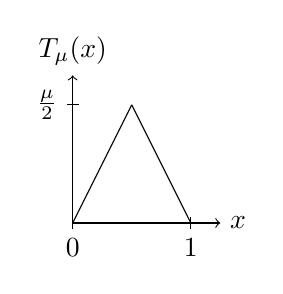
\begin{tikzpicture}[scale=1.5]
      \draw[->] (0.0,0.0) -- (1.25,0.0) node[right] {$x$};  
      \draw[->] (0.0,0.0) -- (0.0,1.25) node[above] {$T_\mu(x)$};
      \draw (0.0,0.0) -- (0.5,1.0);  
      \draw (0.5,1.0) -- (1.0,0.0);
      \draw (0,0.05) -- (0,-0.05) node[below] {$0$};
      \draw (1,0.05) -- (1,-0.05) node[below] {$1$};
      \draw (0.05,1.0) -- (-0.05,1.0) node[left] {$\frac{\mu}{2}$};
\end{tikzpicture}
\end{figure} 

\begin{itemize}
    \item Fiksna točka $x=0$
    \item Fiksna točka $x=\frac{\mu}{\mu+1}$ za $\mu \geq 1$
    \item Maksimum $T_\mu(\frac{1}{2}) = \frac{\mu}{2}$
    \item Zvezna
\end{itemize}

\end{frame}


\begin{frame}
\frametitle{Šotorska preslikava}
\framesubtitle{Dinamika za $\mu \leq 1$}

$0 < \mu < 1$

\smallskip

Orbita poljubne točke konvergira k $0$

\vspace{2\baselineskip}

$\mu = 1$

\smallskip

Samo fiksne in predperiodične fiksne točke

\end{frame}


\begin{frame}
\frametitle{Šotorska preslikava}
\framesubtitle{Dinamika za $1 < \mu < 2$}

\emph{Bifurkacijski diagram} -- asimptotično vedenje orbite

\bigskip

\centering
\includegraphics[width=0.5\textwidth]{tent_bifurcation.png}

\end{frame}


\begin{frame}
\frametitle{Šotorska preslikava}
\framesubtitle{Dinamika za $\mu = 2$}

Interval $[0,1]$, surjekcija

\medskip

Podvajanje šotorov

\bigskip

\includegraphics[width=0.9\textwidth]{tent_2.png}

\end{frame}


\begin{frame}
\frametitle{Šotorska preslikava}
\framesubtitle{Dinamika za $\mu = 2$}

\textbf{Trditev.}
Preslikava $T_2^n : [\frac{k}{2^n}, \frac{k+1}{2^n}] \rightarrow [0,1]$ je linearna in bijektivna za vse $0 \leq k \leq 2^n - 1$.

\medskip

\textbf{Posledica.}
Periodične točke $T_2$ so goste v $[0,1]$. Preslikava $T_2$ je topološko tranzitivna in občutljiva na začetne pogoje.

\medskip

\centering
\includegraphics[width=0.7\textwidth]{tent_2.png}

\end{frame}


\begin{frame}
\frametitle{Šotorska preslikava}
\framesubtitle{Dinamika za $\mu > 2$}

Problem: slika intervala $[0,1]$ ni podmnožica $[0,1]$

\bigskip

\centering
\includegraphics[width=0.9\textwidth]{tent_3.png}

\end{frame}


\begin{frame}
\frametitle{Šotorska preslikava}
\framesubtitle{Dinamika za $\mu > 2$}

Ideja: omejimo prostor, na katerem je definirana $T_\mu$

\medskip

$$ \Lambda_n = \set{ x \in [0,1] \mid T_\mu^n(x) \in [0,1] } $$

\medskip

\centering
\includegraphics[width=0.7\textwidth]{tent_3.png}

\end{frame}


\begin{frame}
\frametitle{Šotorska preslikava}
\framesubtitle{Dinamika za $\mu > 2$}

$$ \Lambda_n = \set{ x \in [0,1] \mid T_\mu^n(x) \in [0,1] } $$

\medskip

$$ \Lambda = \bigcap_{n \in \N_0} \Lambda_n $$

\centering
\includegraphics[width=0.6\textwidth]{tent_3.png}

\end{frame}


\begin{frame}
\frametitle{Šotorska preslikava}
\framesubtitle{Dinamika za $\mu > 2$}

\textbf{Definicija.}
Množica $\Gamma \subset \R$ je Cantorjeva množica, če je zaprta in omejena, ne vsebuje intervalov in je vsaka točka iz $\Gamma$ stekališče od $\Gamma$.

$$ \Lambda = \bigcap_{n \in \N_0} \Lambda_n \quad \leftarrow \text{Cantorjeva množica} $$

\centering
\includegraphics[width=0.7\textwidth]{cantor_set.png}

\end{frame}


\begin{frame}
\frametitle{Šotorska preslikava}
\framesubtitle{Dinamika za $\mu > 2$}

\textbf{Definicija.}
Simbolni prostor $0$ in $1$ je množica vseh neskončnih zaporedij $0$ in $1$, $$ \Sigma_2 = \set{0,1}^{\N_0} = \set{ (s_n)_{n \in \N_0} \mid s_i \in \set{0,1} \; \forall i \in \N_0 }. $$

\bigskip

Na $\Sigma_2$ vpeljemo metriko $$ d(s,t) = \sum_{n \in \N_0} \frac{\vert s_n - t_n \vert}{2^n}. $$

\end{frame}


\begin{frame}
\frametitle{Šotorska preslikava}
\framesubtitle{Dinamika za $\mu > 2$}

\textbf{Definicija.}
Pomik je preslikava $\sigma: \Sigma_2 \rightarrow \Sigma_2$, $$ \sigma(s_0 s_1 s_2 \dots) = s_1 s_2 s_3 \dots $$

\bigskip

\textbf{Izrek.}
Pomik $\sigma$ je kaotična preslikava na $\Sigma_2$.

\end{frame}


\begin{frame}
\frametitle{Šotorska preslikava}
\framesubtitle{Dinamika za $\mu > 2$}

Naj bo $I=[0,1]$ ter označimo $I_0 = [0, \frac{1}{\mu}]$ in  $I_1 = [1 - \frac{1}{\mu}, 1]$. Vpeljimo preslikavo $\Psi: \Lambda \rightarrow \Sigma_2$,
\begin{equation*}
    x \mapsto s_0 s_1 s_2 \dots, \text{ kjer } s_n =
    \begin{cases}
        0 \quad \text{če } T_{\mu}^n(x) \in I_0 \\
        1 \quad \text{če } T_{\mu}^n(x) \in I_1
    \end{cases}.
\end{equation*}

\end{frame}


\begin{frame}
\frametitle{Šotorska preslikava}
\framesubtitle{Dinamika za $\mu > 2$}

\begin{equation*}
    \Psi: \Lambda \rightarrow \Sigma_2, \; x \mapsto s_0 s_1 s_2 \dots, \; s_n =
    \begin{cases}
        0 \quad \text{če } T_{\mu}^n(x) \in I_0 \\
        1 \quad \text{če } T_{\mu}^n(x) \in I_1
    \end{cases}
\end{equation*}

\bigskip

\textbf{Izrek.}
Preslikava $\Psi$ je topološka konjugacija med $(\Lambda, T_\mu)$ in $(\Sigma_2, \sigma)$.

\bigskip

\textbf{Izrek.}
Diskretni dinamični sistem $(\Lambda, T_\mu)$ je kaotičen za $\mu > 2$.

\end{frame}

\end{document}
